%% ****** Start of file apstemplate.tex ****** %
%%
%%
%%   This file is part of the APS files in the REVTeX 4.2 distribution.
%%   Version 4.2a of REVTeX, January, 2015
%%
%%
%%   Copyright (c) 2015 The American Physical Society.
%%
%%   See the REVTeX 4 README file for restrictions and more information.
%%
%
% This is a template for producing manuscripts for use with REVTEX 4.2
% Copy this file to another name and then work on that file.
% That way, you always have this original template file to use.
%
% Group addresses by affiliation; use superscriptaddress for long
% author lists, or if there are many overlapping affiliations.
% For Phys. Rev. appearance, change preprint to twocolumn.
% Choose pra, prb, prc, prd, pre, prl, prstab, prstper, or rmp for journal
%  Add 'draft' option to mark overfull boxes with black boxes
%  Add 'showkeys' option to make keywords appear
%\documentclass[aps,prl,preprint,groupedaddress]{revtex4-2}
\documentclass[aps,prl,preprint,superscriptaddress]{revtex4-2}
%\documentclass[aps,prl,reprint,groupedaddress]{revtex4-2}

% You should use BibTeX and apsrev.bst for references
% Choosing a journal automatically selects the correct APS
% BibTeX style file (bst file), so only uncomment the line
% below if necessary.
%\bibliographystyle{apsrev4-2}

\usepackage{amsmath}
\usepackage{amssymb}
\usepackage{graphicx}
\usepackage{caption}
\usepackage{subcaption}
\usepackage{float}


\begin{document}

% Use the \preprint command to place your local institutional report
% number in the upper righthand corner of the title page in preprint mode.
% Multiple \preprint commands are allowed.
% Use the 'preprintnumbers' class option to override journal defaults
% to display numbers if necessary
%\preprint{}

%Title of paper
%\title{Fitting Room-Temperature Monolayer MoS\textsubscript{2} Electron Hole Liquid Photoluminescence Data with Lorentzian-Broadened Fermi Liquid Theory}

\title{Valley Populations in Indirect-Gap EHL: Using Fermi Liquid Theory to model 1L-MoS2 Phase Transition}

% repeat the \author .. \affiliation  etc. as needed
% \email, \thanks, \homepage, \altaffiliation all apply to the current
% author. Explanatory text should go in the []'s, actual e-mail
% address or url should go in the {}'s for \email and \homepage.
% Please use the appropriate macro foreach each type of information

% \affiliation command applies to all authors since the last
% \affiliation command. The \affiliation command should follow the
% other information
% \affiliation can be followed by \email, \homepage, \thanks as well.
\author{R. L. Wilmington}
\email[]{rlwilmin@ncsu.edu}
\affiliation{Department of Physics, North Carolina State University,
Raleigh, North Carolina 27695-8202, USA}

\author{H. Ardekani}
\affiliation{Department of Physics, North Carolina State University,
Raleigh, North Carolina 27695-8202, USA}

\author{A. Rustagi}
\affiliation{Department of Physics, North Carolina State University,
Raleigh, North Carolina 27695-8202, USA}

\author{A. F. Kemper}
\affiliation{Department of Physics, North Carolina State University,
Raleigh, North Carolina 27695-8202, USA}

\author{R. A. Younts}
\affiliation{NIWC Atlantic}

\author{A. Bataller}
\affiliation{North Carolina State University}

\author{K. Gundogdu}
\affiliation{Department of Physics, North Carolina State University,
Raleigh, North Carolina 27695-8202, USA}

%\homepage[]{Your web page}
%\thanks{}
%\altaffiliation{}

%Collaboration name if desired (requires use of superscriptaddress
%option in \documentclass). \noaffiliation is required (may also be
%used with the \author command).
%\collaboration can be followed by \email, \homepage, \thanks as well.
%\collaboration{}
%\noaffiliation

\date{\today}

\begin{abstract}
[INSERT ABSTRACT HERE]
\end{abstract}

\maketitle

%%%%%%%%%~~~~~~~~~~~~~~~~~~~~~~~~~~~~~~~~~~~~~~~~~~~~~~~~~~~~~~%%%%%%%%%
\section{Introduction\label{Intro}}
%%%%%%%%%~~~~~~~~~~~~~~~~~~~~~~~~~~~~~~~~~~~~~~~~~~~~~~~~~~~~~~%%%%%%%%%


(1) PL data for EHL in 2D MoS2 shows redshift and increase in PL intensity with increased fluence. Band structure calculations show indirect gap transition. (FIG 1)

(2) Possible explanation for intensity increase, redshift: recombination with greater efficiency, charges migrating to Gamma valley following indirect bandgap transition

(3) Additional long low energy tail possibly due to intraband relaxation

(4) Use Fermi liquid theory to develop model to use PL data and band structure calculations to examine efficiency of recombination, evolution of charge carriers between bands, and intraband relaxation times





%%%%%%%%%~~~~~~~~~~~~~~~~~~~~~~~~~~~~~~~~~~~~~~~~~~~~~~~~~~~~~~%%%%%%%%%
\section{Photoluminescence Model}
%%%%%%%%%~~~~~~~~~~~~~~~~~~~~~~~~~~~~~~~~~~~~~~~~~~~~~~~~~~~~~~%%%%%%%%%

\subsection{Overview}

\begin{figure}[H]
	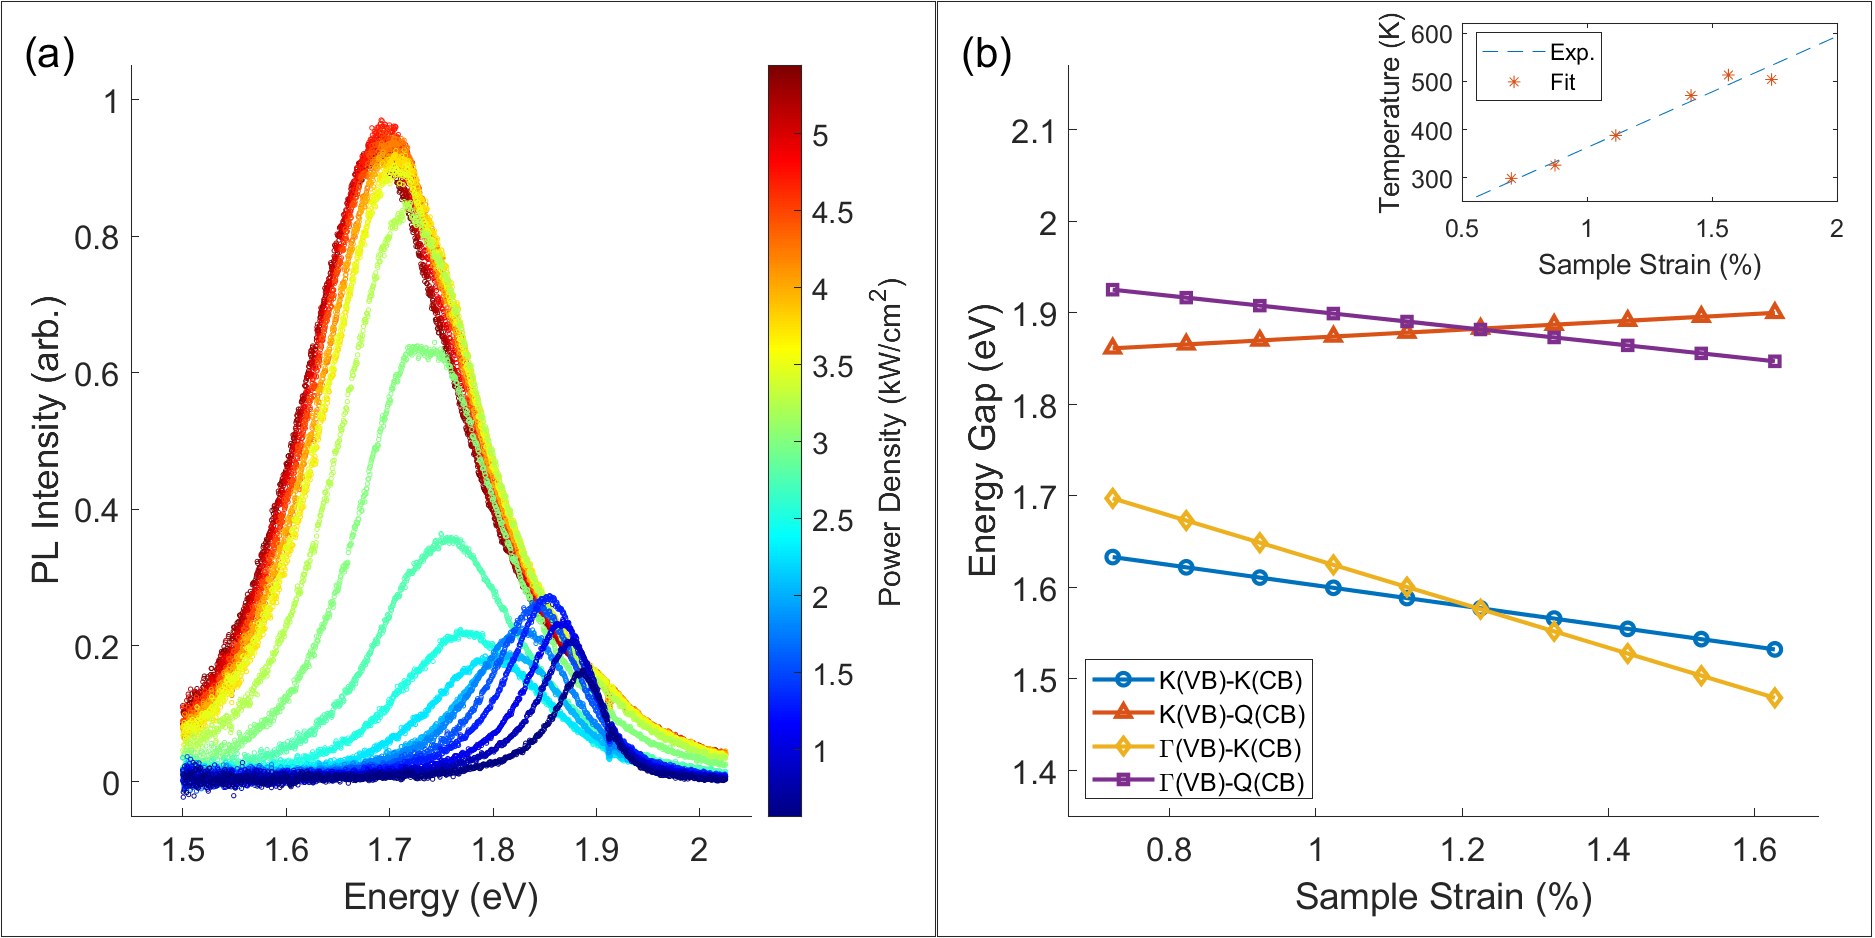
\includegraphics[width=0.95\linewidth]{fig_fig1.png}
	\caption{(a) Photoluminescence showing excitonic to EHL transition in MoS\textsubscript{2}. (b) Calculated shifts in band structure due to sample strain (referenced to valence band K-point)}
	\label{fig:schematic}
\end{figure}

As shown in figure \ref{fig:schematic}, Photoluminescence (PL) data on monolayer MoS\textsubscript{2} samples shows a stark increase in intensity and decrease in peak energy when incident laser power density is increased. Raman spectroscopy and (Avinash methods?) calculations additionally confirm that when laser fluence increases, laser heating causes the lattice to expand. Strain from lattice expansion causes both the $K$-$K$ and $K$-$\Gamma$ energy gaps to decrease, but at approximately 1.2\% strain, the indirect $K$-$\Gamma$ gap becomes smaller than the direct $K$-$K$ gap, resulting in a direct-indirect bandgap semiconductor transition. In summary, as incident CW laser power density is increased, laser heating causes strain, which in turn leads to a band structure transition from a direct to indirect bandgap.

It is possible to estimate the sample temperature by using the relationship between sample strain and temperature, which has also been calculated (PLOT INSET?) using (Avinash Methods). Alternatively, if the sample temperature can be supplied as a fitting parameter, the corresponding band structure can now be computed via the sample strain. Furthermore, the effective mass for each valley can also be calculated as a function of strain, and therefore temperature. Combining these relationships allows the sample temperature to be an effective input parameter to model the electronic behavior of the system. For example, this allows the 2D semiconductor density of states to be written indirectly as a function of temperature:

\begin{equation} \label{2D density of states}
g_{e,h} = \frac{\eta m_{e,h}^*}{\pi \hbar^2}
\end{equation}

where $\eta$ is the degeneracy of the band, and $m^*$ is the corresponding effective mass. Via these methods, the charge carrier density and temperature can be used as fitting parameters from which the strain, effective masses, and band structure can be calculated to predict the PL response over many fluences, and compare it to the PL data.

\subsection{Functional Form}

To relate the calculated band structure transition to the PL data, we developed a model based on well-established fermi liquid theory calculations. The general form for the PL of an EHL can be written as follows (CITE):

\begin{equation} \label{PL Intensity}
I(h\nu) \sim \int_0^{\overline{h\nu}} D_e(E) D_h(\overline{h\nu} - E) dE
\end{equation}

\begin{equation} \label{Energy Offset}
\overline{h\nu} = h\nu - (E_{opt} + E_{bind} - \Delta E_T - \Delta E_{BGR})
\end{equation}

Here $I$ indicates intensity, $D_{e,h}$ is the fermi function-weighted density of states for electrons/holes, $E_{opt}$ is the optical band gap (1.89eV), $E_{bind}$ is the exciton binding energy (0.43eV), $E_T$ is the thermal offset energy, and $E_{BGR}$ is the bandgap renormalization energy (CITE). The optical gap and the exciton binding energy are constant, and the thermal offset energy can be calculated by measuring relative shifts in the calculated band structure as a function of temperature. The bandgap renormalization energy is a correction to the energy bandgap resulting from the high charge carrier density deforming the band. It is included as a fit parameter.


\subsection{Low Energy Tail}

\begin{figure}
	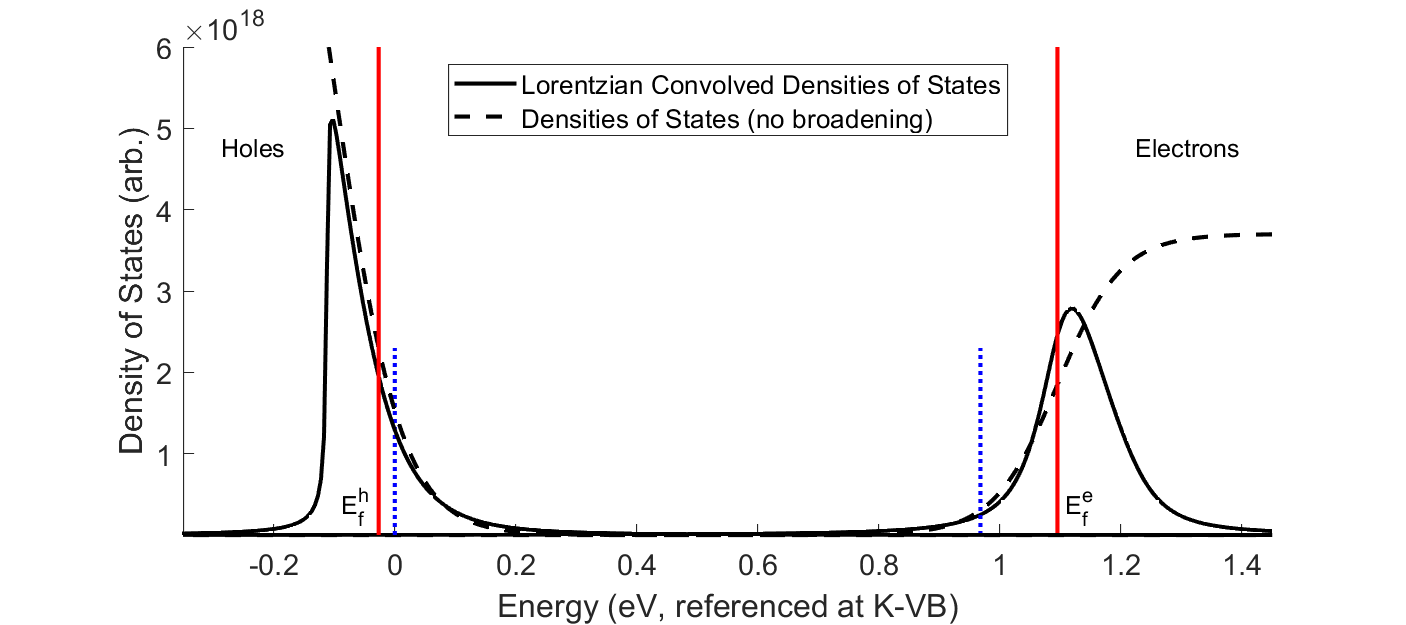
\includegraphics[width=1\linewidth]{fig_DOS.png}
	\caption{Densities of States for holes (left) and electrons (right) referenced from $\Gamma-VB$. Shown with and without Lorentzian convolution. Blue dotted line indicates the indirect semiconductor band gap after laser heating.}
	\label{fig:DOS}
\end{figure}

The simple form of equation 2 yields a reasonable fit to the experimental data, however only on the high energy side. This is a result of the prevalence of transitions within the band. To account for energy broadening due to intraband relaxation of charge carriers, the densities of states for electrons and holes can be convolved with a Lorentzian term (CITE). The resulting prescription to find the weighted density of states for electrons and holes is described below, and visualized in figure \ref{fig:DOS}.

\begin{equation} \label{Lorentzian Convolution}
D_{e,h}(E) = g_{e,h} \int_{-\infty}^\infty f_{e,h}(E') \mathcal{L}(E - E') dE'
\end{equation}

\begin{equation} \label{Lorentzian Term}
\mathcal{L}(E - E') = \frac{1}{2\pi} \frac{\Gamma^{e,h}(E')}{(E - E')^2 + (\frac{1}{2} \Gamma(E'))^2}
\end{equation}

Here $f_{e,h}$ is the fermi function. To first order, the $\Gamma$ broadening parameter will depend quadratically on energy, resulting from the single particle excitation lifetime $\sim w^2$ (CITE). As the energy approaches $E_f$, the broadening reduces to zero. However, to account for sample impurities, finite temperature, and non-constant effective mass, a constant offset parameter has been included:

\begin{equation} \label{Gamma factor}
\Gamma^{e}(E') = \alpha(E' - E_f^{e})^2 + C
\end{equation}

\begin{equation} \label{Gamma factor}
\Gamma^{h}(E') = \beta(E' - E_f^{h})^2 + D
\end{equation}

Note, other slight variations on this broadening function were also considered, producing similar results (see Supplemental Materials).

%%%%%%%%%~~~~~~~~~~~~~~~~~~~~~~~~~~~~~~~~~~~~~~~~~~~~~~~~~~~~~~%%%%%%%%%
\section{Results and Discussion}
%%%%%%%%%~~~~~~~~~~~~~~~~~~~~~~~~~~~~~~~~~~~~~~~~~~~~~~~~~~~~~~%%%%%%%%%

\subsection{Overview}

\begin{figure}
	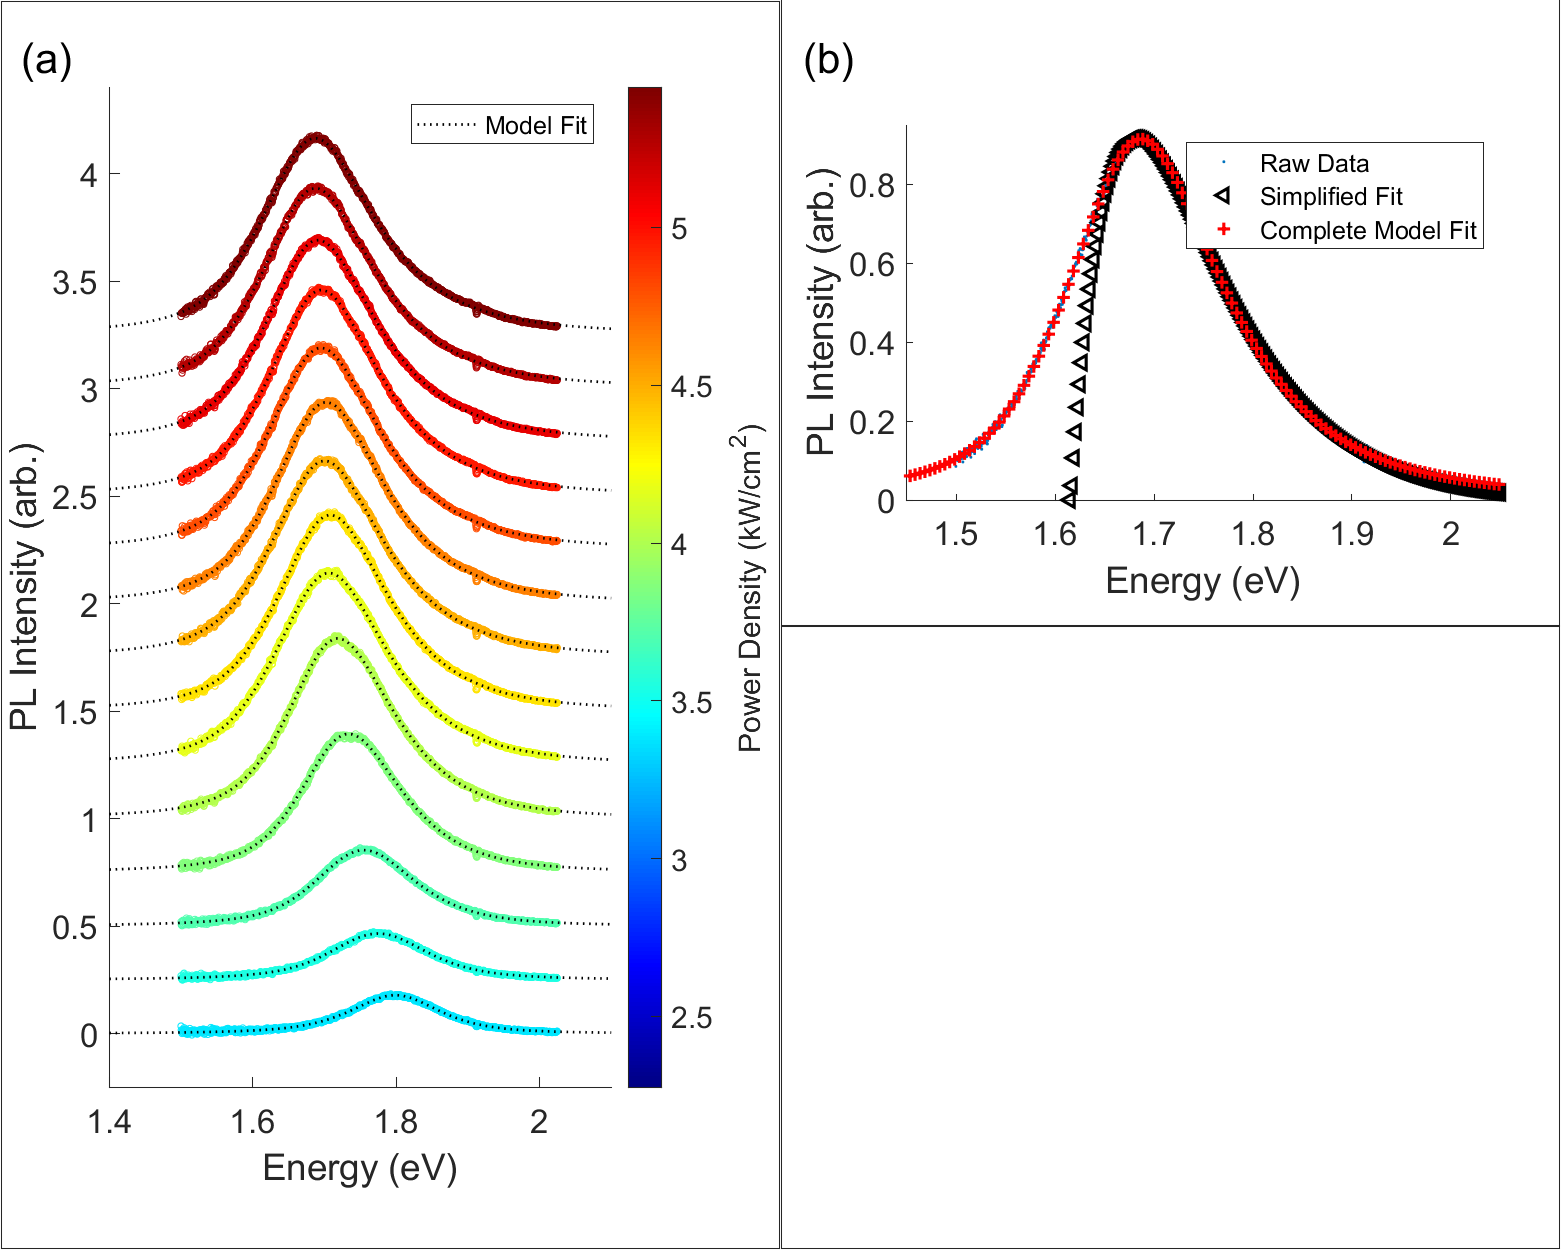
\includegraphics[width=1\linewidth]{fig_fitwith&withoutL.png}
	\caption{Waterfall plot of model fits vs experimental data. (a) Fit calculated using densities of states convolved with a Lorentzian to account for broadening due to intraband transitions. (b) Fit calculated with no intraband transition effects included.}
	\label{fig:result_data}
\end{figure}


To fit the model to the data we used a MATLAB non-linear least squares optimization script using eight fitting parameters: charge carrier density, temperature, bandgap renormalization energy, four Lorentzian broadening parameters, and an overall scaling term. The fitted curve is plotted over the raw data in figure \ref{fig:result_data}. (PLOT INSET: Low fluence model breakdown?) The EHL PL model produces a reasonable fit to the data for the high fluence regime where the system is understood to be in the EHL phase, and well models the transition in the PL peak from approximately $2$-$3kW/cm^2$. However, for low fluences (below $2kW/cm^2$), the system is largely excitonic and the PL model begins to break down (CITE).


\begin{figure}
	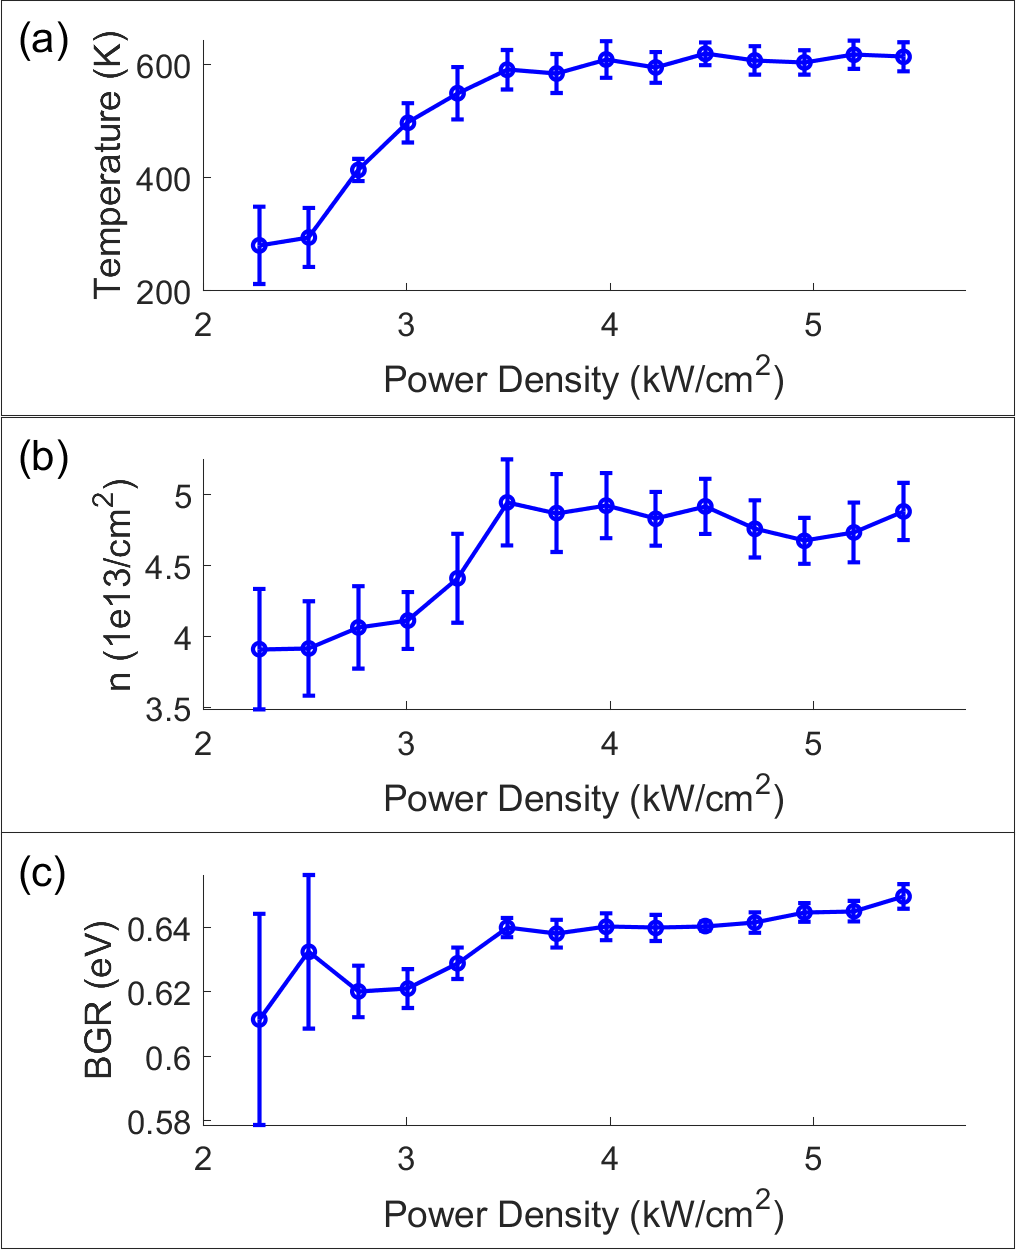
\includegraphics[width=0.5\linewidth]{fig_pars.png}
	\caption{(a) Temperature, (b) Charge carrier density $n$, and (c) bandgap renormalization energy plotted against CW laser power density. Saturation occurs at roughly $3.5 kW/cm^2$. Error bars indicate $2\sigma$ calculated via Monte Carlo error estimation techniques.}
	\label{fig:pars}
\end{figure}

As indicated by the raw PL data, figure \ref{fig:pars} show the sample clearly reaches charge carrier saturation near $3.5 kW/cm^2$, reaching a peak charge carrier density between $4.5$ and $5\times 10^{13}  cm^{-2}$. This agrees well with our previous estimates of the carrier density at $4 \times 10^{13}  cm^{-2}$ (CITE). At the same fluence as the charge carrier saturation, the temperature also appears to reach a maximum. Due to the use of temperature to calculate strain, it is possible that this value indicates a maximum achievable sample strain, and that for temperatures beyond $600 K$, the relationship between strain and temperature does not hold. The bandgap renormalization, dependent on the charge carrier density, also saturates around the same fluence. This corresponds to the qualitative observation that the redshift of the PL peak occurs up until about $3.5 kW/cm^2$, as shown in figure \ref{fig:schematic}. Past that fluence, the temperature (and therefore strain) has reach a maximum, and the charge carriers density is saturated, so any further thermal offset or BGR offset is suppressed, and the peak energy stabilizes. For more discussion on the relationship between the charge carrier density and BGR, see the Supplemental Materials.


\subsection{Charge Carrier Evolution}

\begin{figure}
	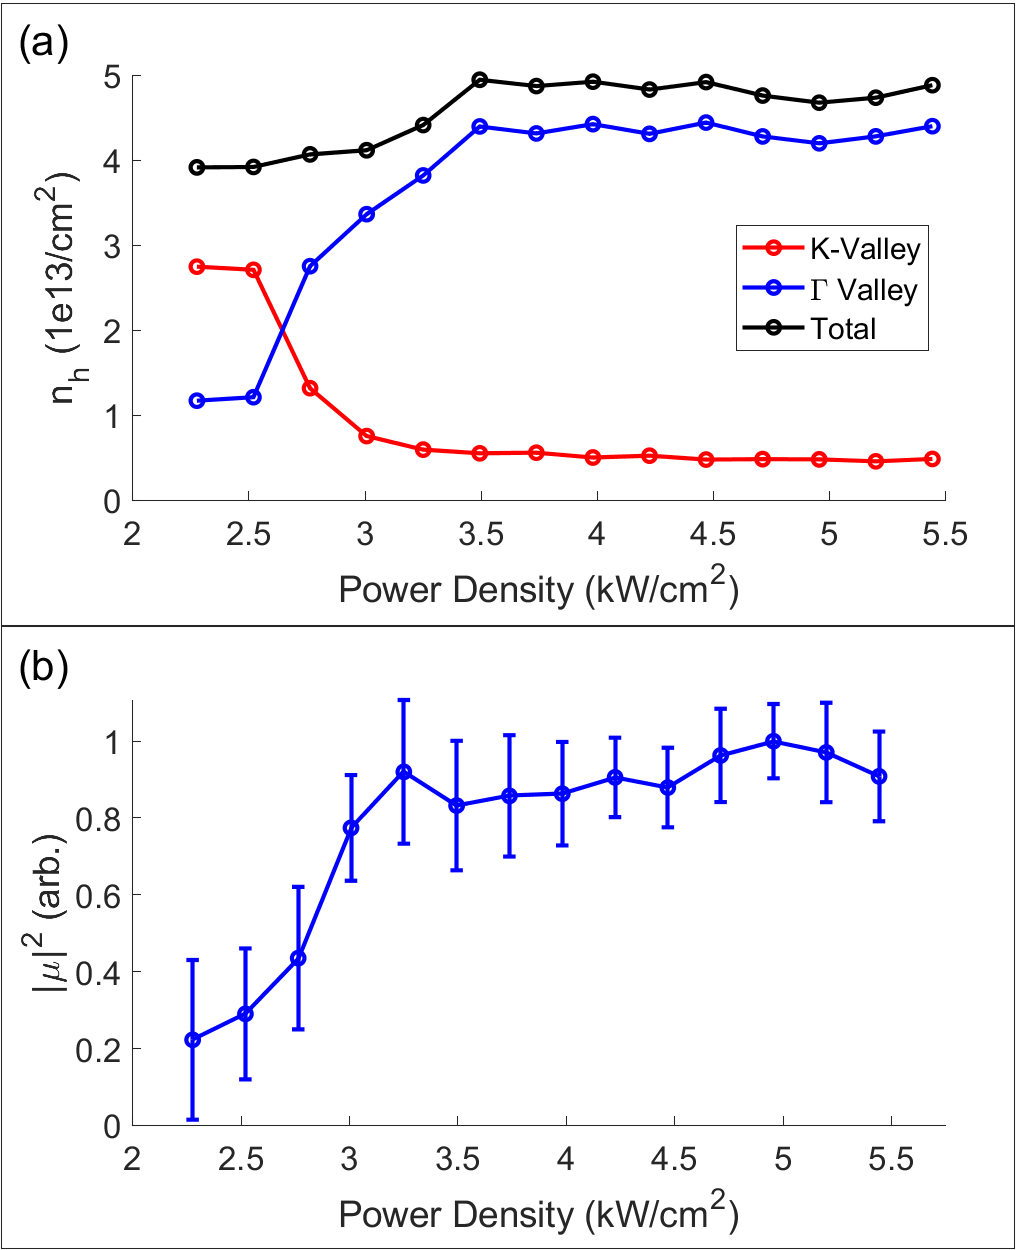
\includegraphics[width=0.5\linewidth]{fig_npervalley+dipole.png}
	\caption{Squared magnitude of the dipole transition moment ($\mu$) and hole charge carrier density per valley ($n_h$)plotted against CW laser power density. Error bars indicate $2\sigma$ calculated via Monte Carlo error estimation techniques.}
	\label{fig:n}
\end{figure}


Using the fitted charge carrier density and temperature, the quasi-fermi levels for electrons and holes can be calculated. Also, the temperature allows the strain and therefore the energy offset between the $K$ and $\Gamma$ valleys to be calculated. Combining these quantities allows the individual populations of charge carriers in each valley to be found, as shown in figure \ref{fig:n}. For low fluences, when the bandgap is direct, holes exist mostly in the $K$ valley, however when the bandgap becomes indirect, the hole population shifts to predominatly rest in the $\Gamma$ valley, where both valleys reach a saturation charge carrier density. By simply looking at the PL intensity, it would be reasonable to suggest that the bandgap is becoming more direct, increasing the electron-hole recombination rate and increasing the PL intensity. However, this finding supports the hypotheses that despite the increase in PL intensity, the phase transition visible in the PL data actually corresponds to the migration of holes from the direct to the indirect gap, as the sample is moving from an excitonic to EHL phase.

\subsection{Dipole Transition Moment}

The proposal that the phase transition observed in the PL data indicates an increase in the density of indirect gap charge carriers necessitates another question: if the bandgap is becoming more indirect (not less), then what explains the increase in PL intensity? To probe this, we can consider the impact of the dipole transition rate of the direct gap recombination.

The basic model for predicting PL response, equation 2, is often cited without a front factor, assuming all constants scaling the PL response will be irrelevant as the exact efficiency of the detection apparatus is unknown. However, we can consider the full expression:

\begin{equation} \label{PL Intensity}
I(h\nu) = A |\mu|^2 \int_0^{\overline{h\nu}} D_e(E) D_h(\overline{h\nu} - E) dE
\end{equation}


where $A$ is the overall scaling factor, including the detector efficiency, and $\mu$ is the dipole transition moment, or rather the matrix element of the quantum-mechanical transition for the direct gap photon emission event (ADD: mu mathematical definition?). This factor can be considered a constant for many systems, but only if the periodic crystal potential is unchanged. The band structure transformation from an indirect to direct bandgap semiconductor, the heating and expansion of the crystal lattice, and the phase transition from a free excitonic gas to a condensed electron hole liquid all contribute to changes in the periodic crystal potential. In particular, to treat the electrons and holes of the EHL phase as "free particles" with effective masses, it is necessary to include effects from neighboring particles as part of the periodic crystal potential, so necessarily the potential for the EHL phase and excitonic phase cannot be the same.

By analyzing the overall front factor of the EHL PL model fit, we can estimate the change to the transition dipole moment as a function of fluence, shown in figure \ref{fig:n}. As carriers migrate to the indirect gap, the remaining direct gap carriers in the $K$-$K$ band provide an increase in the transition dipole moment, indicating the increase in PL observed after the EHL phase transition is a result of a higher probability of charge carrier recombination in the direct gap in the EHL phase.


\subsection{Intraband Relaxation of Charge Carriers}

The inclusion of Lorentzian broadening due to intraband relaxation of charge carriers clearly improves the model fit. With the Lorentzian convolution to the density of states, both the high and low energy tails match well to the raw PL data. This indicates that a major contribution to the PL spectra is from transitions of charges within the band filling vacancies left by other interband transitions. These intraband relaxations can be characterized by the inverse of the Lorentzian broadening parameter used to fit them, which is on the order of the intraband relaxation time, $\Gamma \approx \hbar/\tau$. At saturation, the intraband relxation times for electrons and holes are calculated to be 4.73 fs and 89.66 fs, respectively.





%%%%%%%%%~~~~~~~~~~~~~~~~~~~~~~~~~~~~~~~~~~~~~~~~~~~~~~~~~~~~~~%%%%%%%%%
\section{Conclusion}
%%%%%%%%%~~~~~~~~~~~~~~~~~~~~~~~~~~~~~~~~~~~~~~~~~~~~~~~~~~~~~~%%%%%%%%%


[INSERT CONCLUSION]



\clearpage

%%%%%%%%%~~~~~~~~~~~~~~~~~~~~~~~~~~~~~~~~~~~~~~~~~~~~~~~~~~~~~~%%%%%%%%%
\section{Supplemental Materials}
%%%%%%%%%~~~~~~~~~~~~~~~~~~~~~~~~~~~~~~~~~~~~~~~~~~~~~~~~~~~~~~%%%%%%%%%

\subsection{Additional Fit Outputs}





\begin{figure}[H]
	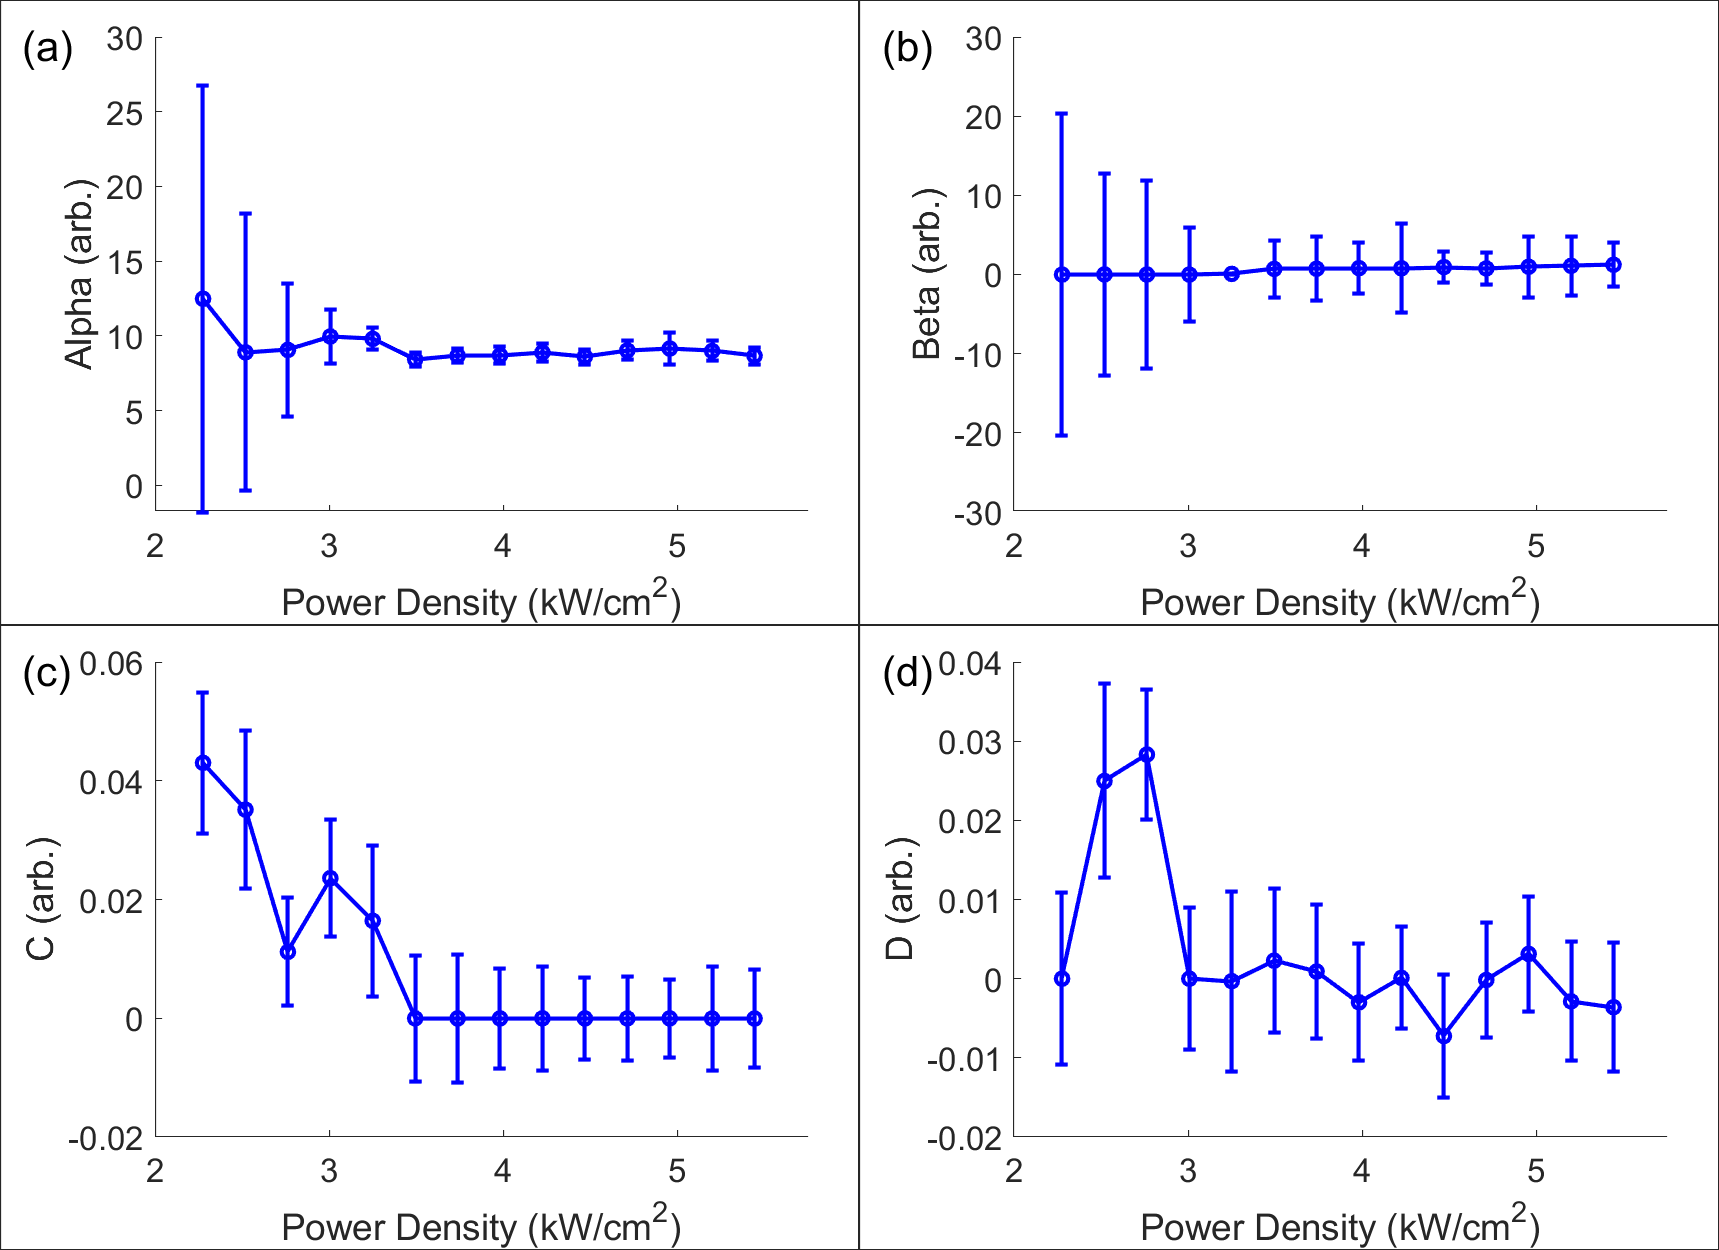
\includegraphics[width=1\linewidth]{fig_alphabetaCD.png}
	\caption{Lorentzian coefficients (alpha (a) and C (c): electrons, beta (b) and D (d): holes) plotted against CW laser power density. Error bars indicate $2\sigma$ calculated via Monte Carlo error estimation techniques.}
	\label{fig:alphabetaCD}
\end{figure}

The Lorentzian fit coefficients include two quadratic terms (alpha, beta) and two constant offsets (C,D) for electrons and holes, respectively. Their values per fluence are reported in figure \ref{fig:alphabetaCD}.

\begin{figure}[H]
	\begin{centering}
		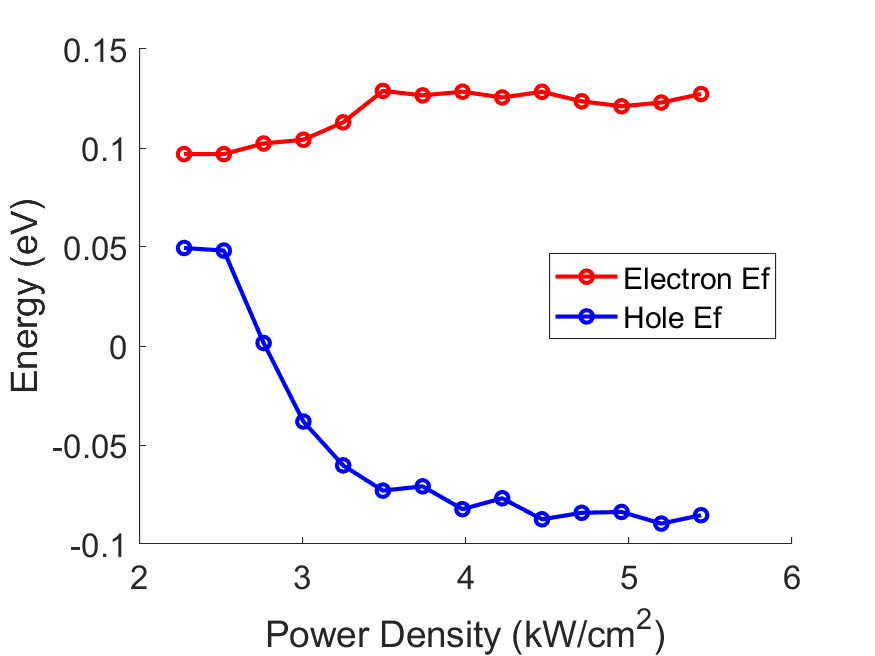
\includegraphics[width=0.5\linewidth]{fermilevelvfluence.png}
		\caption{Quasi-fermi levels for electrons and holes plotted against CW laser power density. Error bars indicate $2\sigma$ calculated via Monte Carlo error estimation techniques.}
		\label{fig:fermilevelvfluence}
	\end{centering}
\end{figure}

Quasi-fermi levels were calculated to compute the charge carrier densities per valley. They are plotted vs fluence in figure \ref{fig:fermilevelvfluence}.

\subsection{Alternative Lorentzian Gamma Expressions}

For the model fit, we used the following energy-dependent forms for the Lorentzian $\Gamma$:

\begin{equation} \label{Gamma factor alternative 1}
	\begin{aligned}
	&\Gamma^{e}(E') = \alpha(E' - E_f^{e})^2 + C \\
	&\Gamma^{h}(E') = \beta(E' - E_f^{h})^2 + D
	\end{aligned}
\end{equation}

However, we also considered both a combined electron/hole form:

\begin{equation} \label{Gamma factor alternative 2}
\Gamma^{e,h}(E') = \alpha(E' - E_f^{e,h})^2 + C
\end{equation}

and a form that only included quadratic coefficients (neglecting $T > 0$ effects):

\begin{equation} \label{Gamma factor alternative 3}
	\begin{aligned}
	&\Gamma^{e}(E') = \alpha(E' - E_f^{e})^2 \\
	&\Gamma^{h}(E') = \beta(E' - E_f^{h})^2
	\end{aligned}
\end{equation}

These alternative forms resulted in very similar model fit outputs.


\subsection{Relating Bandgap Renormalization Energy to Charge Carrier Density}

For our model, we chose to leave charge carrier density and $E_BGR$ as independent fit parameters, however a functional relationship between these two quantities has been proposed (CITE). The bandgap renormalization energy can be related to the charge carrier density by the relation in equation 8:

\begin{equation}
E_{BGR} = C \cdot (n a^2)^{1/3} \cdot E_bind
\end{equation}

where $C$ is an empirical front factor (2.6), $n$ is the charge carrier density, $a$ is the exciton Bohr radius (0.65nm), and $E_bind$ is the exciton binding energy (0.43eV) (CITE). Here is how our model fits compare to the theoretical relationship.

\begin{figure}[H]
	\begin{centering}
	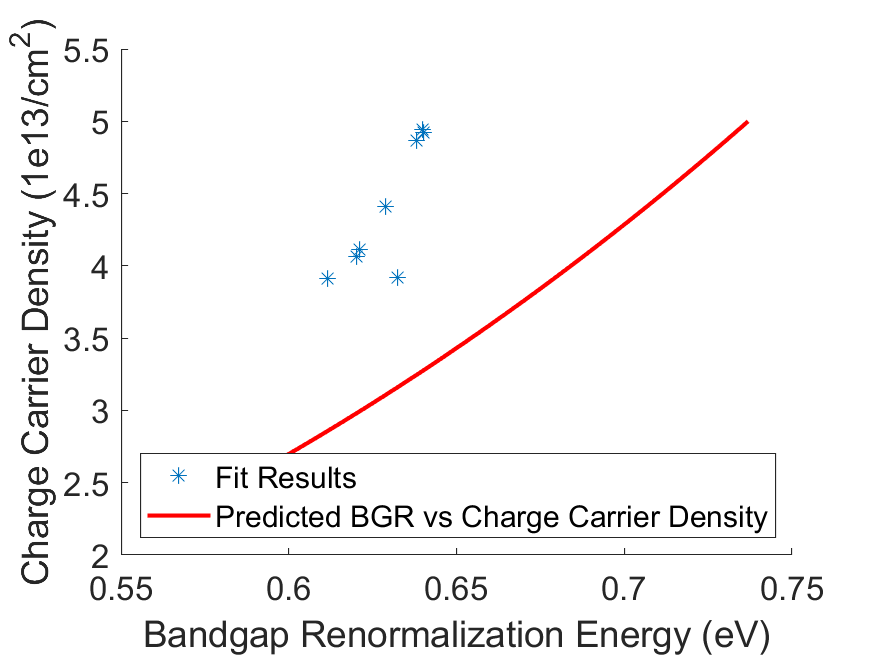
\includegraphics[width=0.5\linewidth]{fig_nvsBGR.png}
	\caption{Comparing predicted relationship of charge carrier density and bandgap renormalization (equation 8) vs fit results.}
	\label{fig:nvsBGR}
	\end{centering}
\end{figure}


% If in two-column mode, this environment will change to single-column
% format so that long equations can be displayed. Use
% sparingly.
%\begin{widetext}
% put long equation here
%\end{widetext}

% figures should be put into the text as floats.
% Use the graphics or graphicx packages (distributed with LaTeX2e)
% and the \includegraphics macro defined in those packages.
% See the LaTeX Graphics Companion by Michel Goosens, Sebastian Rahtz,
% and Frank Mittelbach for instance.
%
% Here is an example of the general form of a figure:
% Fill in the caption in the braces of the \caption{} command. Put the label
% that you will use with \ref{} command in the braces of the \label{} command.
% Use the figure* environment if the figure should span across the
% entire page. There is no need to do explicit centering.

% \begin{figure}
% \includegraphics{}%
% \caption{\label{}}
% \end{figure}

% Surround figure environment with turnpage environment for landscape
% figure
% \begin{turnpage}
% \begin{figure}
% \includegraphics{}%
% \caption{\label{}}
% \end{figure}
% \end{turnpage}

% tables should appear as floats within the text
%
% Here is an example of the general form of a table:
% Fill in the caption in the braces of the \caption{} command. Put the label
% that you will use with \ref{} command in the braces of the \label{} command.
% Insert the column specifiers (l, r, c, d, etc.) in the empty braces of the
% \begin{tabular}{} command.
% The ruledtabular enviroment adds doubled rules to table and sets a
% reasonable default table settings.
% Use the table* environment to get a full-width table in two-column
% Add \usepackage{longtable} and the longtable (or longtable*}
% environment for nicely formatted long tables. Or use the the [H]
% placement option to break a long table (with less control than 
% in longtable).
% \begin{table}%[H] add [H] placement to break table across pages
% \caption{\label{}}
% \begin{ruledtabular}
% \begin{tabular}{}
% Lines of table here ending with \\
% \end{tabular}
% \end{ruledtabular}
% \end{table}

% Surround table environment with turnpage environment for landscape
% table
% \begin{turnpage}
% \begin{table}
% \caption{\label{}}
% \begin{ruledtabular}
% \begin{tabular}{}
% \end{tabular}
% \end{ruledtabular}
% \end{table}
% \end{turnpage}

% Specify following sections are appendices. Use \appendix* if there
% only one appendix.
%\appendix
%\section{}

% If you have acknowledgments, this puts in the proper section head.
%\begin{acknowledgments}
% put your acknowledgments here.
%\end{acknowledgments}

% Create the reference section using BibTeX:
\bibliography{basename of .bib file}

\end{document}
%
% ****** End of file apstemplate.tex ******

